\documentclass[11pt]{article}
\usepackage[T1]{fontenc}
\usepackage{lmodern,microtype,amsmath,amssymb,amsthm,mathtools,xurl}
\usepackage[a4paper,margin=28mm]{geometry}
\usepackage{tikz}
\usetikzlibrary{arrows.meta,calc,positioning}
\usepackage[colorlinks=true,linkcolor=blue!55!black,citecolor=blue!55!black,urlcolor=blue!55!black]{hyperref}
\setlength{\emergencystretch}{2em}
\numberwithin{equation}{section}
\newtheorem{theorem}{Theorem}[section]
\newtheorem{proposition}[theorem]{Proposition}
\newtheorem{lemma}[theorem]{Lemma}
\newtheorem{corollary}[theorem]{Corollary}
\theoremstyle{definition}\newtheorem{definition}[theorem]{Definition}
\theoremstyle{remark}\newtheorem{remark}[theorem]{Remark}
\newcommand{\Turn}{\mathcal T}
\newcommand{\Vol}{\operatorname{Vol}}
\newcommand{\ii}{\mathrm i}
\title{Ordered tangle reductions and long net twists}
\author{}\date{}
\begin{document}
\maketitle
\begin{abstract}
We give a finite reduction of ordered two-strand tangle expressions that keeps the signed sum and original labels of every fused twist region. For a cylindrical product closure, the surviving label partition is independent of the twist parities; the parities determine the rotations and orders in the resulting presentation. Allowing either closure and vanishing sums gives a tree of explicitly marked connected sums. The reduction uses ambient isotopies with prescribed collars and retains every closed component. Combining it with the volume theorem for strict Conway compositions gives an all-integer-level volume limit whenever the surviving strict factors have sufficiently long net twists and the input knot is hyperbolic. Under the same longness condition the terminal factors also give a finite criterion for hyperbolicity. The original expression is arbitrary but fixed, and longness is imposed on the surviving sums, not on the written summands.
\end{abstract}

\section{The question and the precise input}\label{cr:introduction}

Two large twist regions can cancel. For example, replacing an integral braid $R^a$ by $R^{a+2k}R^{-2k}$ changes neither the tangle nor its closure, while both new written counts tend to infinity with $|k|$. A useful long-twist statement must therefore specify which sums of the original counts survive the tangle operations. We do this before invoking a geometric or quantum theorem.

The constructions belong to the algebraic tangle calculus introduced by Conway~\cite{Conway}. Rational tangles and their flip and flype operations are treated by Kauffman--Lambropoulou~\cite{KL}; the broader arborescent classification is developed by Bonahon--Siebenmann~\cite{BS}. Our reduction keeps the ordered expression and its labelled twist sums. It need not be canonical among all presentations of the same link. In particular, we retain a rotation of an arbitrary subtangle rather than use flip invariance available in special rational cases. Hyperbolicity of much broader arborescent classes is studied by Volz~\cite{Volz}. The argument here needs only the long strict factors furnished by the following companion theorem and an elementary group obstruction to having two such nontrivial summands.

\subsection{Boxes, signs and closures}

Place a two-strand tangle in a ball with four specified boundary points. A tangle consists of two arcs and possibly finitely many closed components. All the latter are part of the link. In the diagram plane label the points
\[
 0=\text{lower left},\quad1=\text{lower right},\quad
 2=\text{upper right},\quad3=\text{upper left}.
\]
Depth is the $y$ coordinate and the vertical stack axis is $z$. The product $FG$ puts $F$ below $G$ and joins $F_2$ to $G_1$ and $F_3$ to $G_0$. Its exposed ordered tuple is $(F_0,F_1,G_2,G_3)$. Products are ordered; brackets may be changed by rescaling the empty stack collars.

The clockwise quarter-turn $\Turn$ is the spatial rotation
\[
             \Turn(x,y,z)=(z,y,-x).
\]
It carries the whole ball, including its closed components. The new endpoint tuple is $(F_1,F_2,F_3,F_0)$. Write $R^n$ for the standard integral two-braid with $n\in\mathbb Z$ signed half twists, and define a labelled elementary piece by
\begin{equation}\label{cr:leaf}
                    h_i(n_i)=\Turn(R^{n_i}).
\end{equation}
Positive and negative powers refer to this one fixed braid convention. A label $i$ occurs exactly once in the expression. Turns and products of the pieces \eqref{cr:leaf} are the allowed operations.

The cylindrical closure $C(E)$ connects $E_0$ to $E_3$ and $E_1$ to $E_2$ by the fixed empty outside arcs. The cap closure $D(E)$ connects $E_0$ to $E_1$ and $E_2$ to $E_3$. Rotating the closed picture identifies
\begin{equation}\label{cr:two-closures}
                         D(E)=C(\Turn E).
\end{equation}
Here and below equality of such diagrams means the displayed actual isotopy class, with these outside arcs. A four-point permutation alone would not specify a closure: one could otherwise insert a boundary Dehn twist.

\subsection{Strict expressions and the imported theorem}

The formal strictness test does not inspect the numerical twist counts. The possible open types are
\[
 L=(0,1/2),\qquad H=(1/2,1),\qquad A=(0,1).
\]
Each formal $h$ has type $L$. A turn exchanges $L,H$ and fixes $A$. The product table is
\begin{equation}\label{cr:type-table}
\begin{array}{c|ccc}
 &L&H&A\\\hline
 L&A&H&A\\
 H&H&\varnothing&H\\
 A&A&H&A
\end{array}
\end{equation}
The allowed closing pairs are $AA,AL,AH,LH$, in either order. An expression $C(FG)$ is \emph{strict} if every product and its closing pair pass this test. The intervals are the possible normalized output states of the positive Newton variational problem. Their exact support interpretation and the equivalence with a strict interior state are \cite[Lemma 2.2 and Theorem 2.5]{Profiles}. This test concerns the written formal expression. A formal piece with count zero still has its formal type; no geometric conclusion for a zero filling follows from that convention.

\begin{proposition}[The strict-volume input]\label{cr:import}
Fix a literal strict expression with at least two leaves. Fix a retained half-twist pattern $\epsilon_i\in\{0,1\}$ whose complete strand pairing, including internal circles, has one component. There is $P_0$ such that every fixed signed integer tuple with $|p_i|>P_0$, and physical crossing powers
\begin{equation}\label{cr:power-slope}
                         n_i=\epsilon_i-2p_i,
\end{equation}
gives a hyperbolic knot $K$ and
\begin{equation}\label{cr:volume-limit}
 \lim_{N\to\infty}\frac{2\pi}{N}\log|K_N(K)|
                          =\Vol(S^3\setminus K).
\end{equation}
The limit includes every sufficiently large integer level. The signs and relative sizes of the $p_i$ are unrestricted, and the tuple and expression are fixed before taking this limit.
\end{proposition}

This is \cite[Theorem 1.1]{Asymptotics}. The invariant $K_N$ is the reduced enhanced Kashaev invariant with unknot value one and the recorded zero-framing normalization; its comparison with the physical evaluation is \cite[Theorem 10.1]{Finite}, at $N\ge3$. All subsequent invariant identities can be restricted to these levels. The missing single level $N=2$ has no bearing on \eqref{cr:volume-limit}. For a fixed strict template $\sigma$, define
\[
 P_\sigma=\max\bigl(\{0\}\cup
   \{P_{\sigma,\epsilon}:\epsilon\text{ gives one component}\}\bigr).
\]
The set of parity patterns is finite; the definition also covers a template admitting no knot-producing pattern. A crossing-weight threshold is
\begin{equation}\label{cr:crossing-threshold}
                         B_\sigma=2P_\sigma+1.
\end{equation}
Indeed $|n_i|>B_\sigma$ implies $|p_i|=|\epsilon_i-n_i|/2>P_\sigma$. This is the only asymptotic input to this paper.

\subsection{The conclusions}

Fix a finite expression on labels $\{1,\ldots,m\}$. For a nonempty block of labels $B$, put
\begin{equation}\label{cr:net}
                         W_B=\sum_{i\in B}n_i.
\end{equation}
A formal piece remembers $B$ even when its evaluated weight is zero.

\begin{theorem}[Ordered product normalization]\label{cr:ordered}
Suppose the input is $\mathcal E=C(FG)$, with $m\ge2$. There is a partition of its original labels into nonempty disjoint blocks. For each original parity vector, a deterministic finite procedure produces either a strict cylindrical product expression on those net blocks, or the integral braid closure $C(R^{\sum_i n_i})$. The partition is independent of the parity vector; the orders and recorded rotations of subexpressions can depend on it. For every integer assignment of that parity, including zero weights and zero sums, the output is ambient isotopic to the input in oriented $S^3$.

There is a finite constant $B(\mathcal E)$ such that, if the output is strict, the input has one component, and every surviving $|W_B|>B(\mathcal E)$, then the input is hyperbolic and satisfies \eqref{cr:volume-limit}.
\end{theorem}

An arbitrary closure may require cap splitting before this theorem applies. It can also lie on a wall where some final net sum vanishes. The next result records these possibilities.

\begin{theorem}[Either closure and zero sums]\label{cr:arbitrary}
Fix a finite expression $E$ with $m\ge1$ and choose $C(E)$ or $D(E)$. A deterministic finite procedure gives an exhibited tree of componentwise connected sums of strict cylindrical product expressions with nonzero net weights, integral braid closures, and unknots. Surviving and deleted net blocks partition the original labels. Only the original parities and the zero/nonzero pattern of their finitely many subset sums choose the output templates.

There is a finite $B_E$ such that the following holds. Suppose the input has one component and every weight on every surviving strict factor has magnitude greater than $B_E$. Then the input is hyperbolic if and only if exactly one terminal factor is strict and all other terminal factors are unknots. In that case it is ambient isotopic to the strict factor and satisfies \eqref{cr:volume-limit}.
\end{theorem}

The condition is on surviving strict weights only. Elementary factors can have small weights. Without the longness condition the decomposition remains valid, but this theorem does not decide the geometry of a short strict factor. Sections~\ref{cr:rotations}--\ref{cr:partition} prove the ordered normalization. Sections~\ref{cr:zeros}--\ref{cr:groups} prove the all-root reduction and its hyperbolic criterion. The last section transports the invariant and volume and states useful numerical sufficient conditions.

\section{Rotations in an actual collar}\label{cr:rotations}

Three proper half-turns will keep track of the order changes:
\begin{equation}\label{cr:rotations-formula}
 \rho(x,y,z)=(-x,-y,z),\quad
 \kappa(x,y,z)=(x,-y,-z),\quad
 \tau(x,y,z)=(-x,y,-z)=\Turn^2(x,y,z).
\end{equation}
Their endpoint permutations are $(01)(23)$, $(03)(12)$ and $(02)(13)$, respectively. Direct composition of these spatial maps gives
\begin{equation}\label{cr:rotation-rules}
\begin{aligned}
 \rho(FG)&=\rho(F)\rho(G),&\rho(\Turn F)&=\Turn\kappa(F),\\
 \kappa(FG)&=\kappa(G)\kappa(F),&\kappa(\Turn F)&=\Turn\rho(F),\\
 \tau(FG)&=\tau(G)\tau(F),&\tau(\Turn F)&=\Turn\tau(F).
\end{aligned}
\end{equation}
The order reverses precisely when the stack coordinate reverses.

Each standard integral braid is fixed by these half-turns, with its signed exponent unchanged. One direct model has its two strand positions at height $z\in[-1,1]$ proportional to
\[
 \pm\bigl(\cos(\pi n(z+1)/2),\sin(\pi n(z+1)/2)\bigr)
\]
in the transverse plane, after a fixed choice of sign convention. Each map in \eqref{cr:rotations-formula} changes the displayed angle only by an integral multiple of $\pi$ after the prescribed height reversal. The unordered pair of strands is therefore unchanged. The same conclusion holds for $h_i=\Turn R^{n_i}$ by \eqref{cr:rotation-rules}. Reversal in the projection is accompanied by the necessary reversal of depth; it does not negate a crossing. Pushing a half-turn through an expression consequently reverses specified product orders but preserves all leaf labels and weights.

\begin{lemma}[Twist sliding]\label{cr:slide}
For every tangle $F$, including its closed components, and every $a,b\in\mathbb Z$,
\begin{equation}\label{cr:slide-formula}
 R^aF\simeq\rho^a(F)R^a,\qquad
                     R^aR^b\simeq R^{a+b}.
\end{equation}
The first isotopy is relative to the four outside endpoints. The symbol $\simeq$ denotes an ambient isotopy, carrying a marked point and any chosen ribbon.
\end{lemma}
\begin{proof}
Put $F$ in a smaller round cylinder inside the box and leave empty collars at both ends. In cylindrical coordinates $(r,\phi,z)$, take smooth cutoffs $\eta(r),\xi(z)$ equal to one on that smaller cylinder and zero near the outside boundary. The maps
\[
 (r,\phi,z)\longmapsto
            (r,\phi+t\pi\eta(r)\xi(z),z),\qquad0\le t\le1,
\]
are homeomorphisms fixed near the boundary: their inverse subtracts the same angle since $r,z$ are unchanged. At the end the inner tangle has rotated by $\rho$. Its two end collars acquire opposite half twists. Choose the angle sign to match $R$. Applying this isotopy to $\rho(F)$ yields $R F\simeq\rho(F)R$. The inverse isotopy and iteration prove the formula for all $a$. Closed components lie inside the rotating cylinder and move with it. The second assertion concatenates equal twists and cancels adjacent opposite crossings by Reidemeister II.
\end{proof}

The rotation $\rho^a$ depends only on $a\bmod2$. An integral factor can thus be moved through an ordered stack, but every factor passed acquires its stated rotation. There is no assertion that open factors commute.

\section{The closing sphere and its ordered moves}\label{cr:closing}

The four connections in $C(FG)$ are exactly
\begin{equation}\label{cr:closing-pairs}
 F_2\leftrightarrow G_1,\quad F_3\leftrightarrow G_0,
 \quad F_0\leftrightarrow G_3,\quad F_1\leftrightarrow G_2.
\end{equation}
The first two are the stack collar and the last two are the empty outside arcs. Straightening these collars with their planar sectors identifies the two tangle-ball boundaries by
\begin{equation}\label{cr:reflection}
            h(x,y,z)=(x,y,-z),\qquad h(i)=3-i.
\end{equation}
This is orientation reversing on the sphere. Although its endpoint permutation equals that of $\kappa$, it is not the proper rotation $\kappa$.

\begin{lemma}[Closed turns and cyclicity]\label{cr:closed-moves}
For the fixed closures,
\begin{align}
 C((\Turn F)G)&\simeq C(F(\Turn G)),\label{cr:turn-transfer}\\
 C((\Turn F)(\Turn G))&\simeq C(F\tau(G)),\label{cr:double-turn}\\
 C(FG)&\simeq C(GF).\label{cr:cyclic}
\end{align}
All rotations on the right are actual rotations of the indicated tangles.
\end{lemma}
\begin{proof}
Let $\Turn_t$ be rotation through $t\pi/2$ in the diagram plane. The specified gluing has
\[
                     h\Turn_t h^{-1}=\Turn_t^{-1}.
\]
Act by $\Turn_t$ on the first ball and by $\Turn_t^{-1}$ on the second. These maps agree under the boundary identification and extend over the balls. They give an isotopy of their glued $S^3$, starting at the identity. Applied to $C(F(\Turn G))$, its endpoint at $t=1$ is $C((\Turn F)G)$. This proves \eqref{cr:turn-transfer}; substituting $\Turn G$ for $G$ gives \eqref{cr:double-turn}. A boundary Dehn twist not present in \eqref{cr:closing-pairs} would change this argument.

For cyclicity put the two successive stack intervals in the standard unknotted solid torus $D^2\times S^1$ and move the cutting section past the first interval. Translation around its circle coordinate gives the isotopy. In the model $S^3\subset\mathbb C^2$, rotation of the corresponding complex coordinate extends this translation to the ambient sphere. The marked point and every component are carried along. This proves only closed cyclicity, as used here.
\end{proof}

\begin{lemma}[Exposing a leaf or junction]\label{cr:expose}
In a cylindrical product closure with at least two labelled leaves, any chosen leaf can be exposed as $C(h_iQ)$. Every other leaf occurs in $Q$ exactly once. Likewise any chosen product junction can be brought to the closing sphere, with its original attached subexpressions in recorded order.
\end{lemma}
\begin{proof}
Regard a selected subtree as the first argument of $C(AQ)$. If $A=BC$ and the target lies in $B$, reassociate to $C(B(CQ))$. If it lies in $C$, use cyclicity to obtain $C(C(QB))$. If $A=\Turn B$, transfer the turn to obtain $C(B(\Turn Q))$. Start by cyclicity if the target lies in the other closing factor. Each step shortens the path to the selected leaf or junction and moves a sibling, never copies it. Stop at that target. Orders and all new turns are given explicitly by these formulas.
\end{proof}

\begin{figure}[ht]
\centering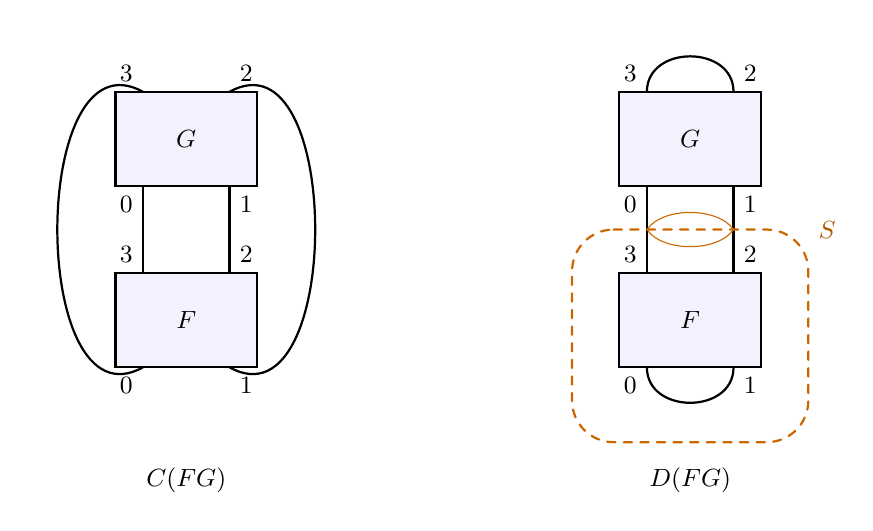
\begin{tikzpicture}[x=1cm,y=1cm,line cap=round,thick,
 every node/.style={font=\small}]
\foreach \dx/\lab in {0/{C(FG)},6.4/{D(FG)}}{
 \begin{scope}[shift={(\dx,0)}]
 \draw[fill=blue!5] (-.9,0) rectangle (.9,1.2);
 \draw[fill=blue!5] (-.9,2.3) rectangle (.9,3.5);
 \node at (0,.6) {$F$};\node at (0,2.9) {$G$};
 \foreach \x in {-.55,.55}{\draw (\x,1.2)--(\x,2.3);}
 \node[below] at (0,-1.15) {$\lab$};
 \node[below left] at (-.55,0) {$0$};
 \node[below right] at (.55,0) {$1$};
 \node[above right] at (.55,1.2) {$2$};
 \node[above left] at (-.55,1.2) {$3$};
 \node[below left] at (-.55,2.3) {$0$};
 \node[below right] at (.55,2.3) {$1$};
 \node[above right] at (.55,3.5) {$2$};
 \node[above left] at (-.55,3.5) {$3$};
 \end{scope}
}
\draw (-.55,0).. controls (-2,-.8) and (-2,4.3)..(-.55,3.5);
\draw (.55,0).. controls (2,-.8) and (2,4.3)..(.55,3.5);
\draw (5.85,0)..controls(5.85,-.6)and(6.95,-.6)..(6.95,0);
\draw (5.85,3.5)..controls(5.85,4.1)and(6.95,4.1)..(6.95,3.5);
\draw[orange!80!black,dashed,rounded corners=15pt]
 (4.9,1.75)--(7.9,1.75)--(7.9,-.95)--(4.9,-.95)--cycle;
\node[right,orange!70!black] at (7.9,1.75) {$S$};
\draw[orange!80!black,thin] (5.85,1.75)..controls(6.05,1.46)and(6.75,1.46)..(6.95,1.75);
\draw[orange!80!black,thin] (5.85,1.75)..controls(6.05,2.04)and(6.75,2.04)..(6.95,1.75);
\end{tikzpicture}

\caption{The prescribed closures of the same lower box $F$ and upper box $G$. The cylindrical closure on the left uses the outside returns of \eqref{cr:closing-pairs}. For the cap closure on the right, a sphere around $F$ and its lower cap meets only the two interface strands. The dashed line is the section of that sphere in the diagram plane. Cutting there creates the upper cap of $F$ and the lower cap of $G$, so the connected-sum components are specified. Endpoint numbers refer to each box before stacking.}\label{cr:closure-figure}
\end{figure}

\section{A terminating ordered normalization}\label{cr:normalization}

A formal leaf now has a nonempty label block $B$ and weight $W_B$. Different live leaves have disjoint blocks. The procedure in this section never tests whether $W_B=0$.

First replace every $\Turn^2$ by $\tau$ and propagate the half-turn through the subtree using \eqref{cr:rotation-rules}. Resolve it on the integral leaves. Reassociate consecutive products into maximal ordered stacks, each with at least two factors. Their factors have the forms
\begin{equation}\label{cr:stack-factors}
              h(B),\qquad \Turn h(B)=R^{W_B},\qquad \Turn(P),
\end{equation}
where $P$ is another maximal stack. The second form is a \emph{direct integral factor}: it is integral at this particular stack, not behind another turn.

Choose a deepest stack with at least two direct integral factors. Slide all those factors to its right end by Lemma~\ref{cr:slide}, then fuse them. The new integral factor carries the union of their blocks and the sum of their weights. Propagate all rotations by \eqref{cr:rotation-rules}, shorten turn chains and flatten adjacent products again. Fix an order for every choice, for example first in the current ordered traversal.

A rotated direct integral remains direct integral; a rotated ordinary leaf remains ordinary; a rotated turned stack remains a turned stack. Consequently this propagation does not hide an integral factor by replacing a rotated arbitrary tangle by the original one. Each fusion decreases the number of live leaves, even if the new sum is zero. Between fusions there are only finitely many turn-shortening and flattening operations, and the propagation visits a finite tree without introducing leaves. The procedure terminates after at most $m-1$ fusions.

\begin{lemma}[The reduced-stack types]\label{cr:reduced-stacks}
When every maximal stack has at most one direct integral factor, every other factor has type $L$ or $A$. A stack with no direct integral has type $A$; a stack with one has type $H$. Any ordered binary resolution of such a stack passes the product table.
\end{lemma}
\begin{proof}
Induct upward from the deepest stacks. Ordinary leaves have type $L$. A child stack has type $A$ or $H$ by induction, so its turn has type $A$ or $L$. At least two $L/A$ factors multiply to $A$. Inserting the single $H$ factor yields $H$, and no intermediate grouping can encounter two $H$ factors. If a stack has collapsed to one factor during fusion, that factor is integral: it results from fusing all the former factors, not from deleting arbitrary subtrees. Suppress this unary stack before applying the induction.
\end{proof}

For the input $C(FG)$ the root is still a product unless all its factors fuse to one integral box. The latter case is the stated elementary output. Otherwise write the normalized maximal root stack with $k\ge2$ factors. If $k\ge3$ and none is integral, expose one $L/A$ factor against the product of the rest, of type $A$. If one is integral, use closed cyclicity to expose it against the other $k-1$ factors, again of type $A$. Both closures pass the table.

When $k=2$, all pairs pass except $LL$. A type-$L$ factor is literally $\Turn U$, where $U$ is either a single integral box or a stack with precisely one direct integral factor. This includes $h(B)=\Turn R^{W_B}$. The failed root therefore has the actual isotopy
\begin{equation}\label{cr:failed-root}
                C((\Turn U)(\Turn V))\simeq C(U\tau V).
\end{equation}
Flattening exposes the one integral from each side, together with $L/A$ factors. Slide and fuse these two integrals, retaining all rotations, and normalize again. This return makes a genuine fusion. Thus the full root procedure terminates too. Zero sums remain named integral boxes; they are not removed in this section.

Each step preserves or unions disjoint label blocks. Fixing the original parities determines the parity of every moved sum and hence every rotation. The entire ordered schedule and the resulting structural expression are therefore fixed on a parity class, even when some sums happen to vanish. This proves the existence and isotopy assertions of Theorem~\ref{cr:ordered}. We next strengthen the bookkeeping by showing that its partition can be chosen independently of parity.

\section{The net blocks before assigning parities}\label{cr:partition}

There is a useful finite graph underlying the normalization. It records tangle operations and turn parity, not a new knot projection. Remove the last closing product and join the output ends of $F$ and $G$. Represent every remaining product by a trivalent vertex. Put a bit in $\{0,1\}$ on each edge recording the number of quarter-turns on it modulo two. A leaf ends at the integral braid $R^{n_i}$, so the turn in $h_i=\Turn R^{n_i}$ contributes one to its leaf-edge bit.

For $m\ge3$ the graph is an unrooted tree with $m$ labelled leaves and internal vertices of valence three. Contract every internal edge with bit zero. This joins associative product regions. The result is a tree of junctions of valence at least three, with bit one on every internal edge. At a junction $v$, call the labels on its bit-zero leaf edges $I_v$. These are exactly its direct integral labels. The partition is
\begin{equation}\label{cr:partition-formula}
 \{I_v:I_v\ne\varnothing\}\ \cup\
 \{\{i\}:\text{the leaf edge at }i\text{ has bit one}\}.
\end{equation}
Every label occurs in exactly one displayed set.

\begin{proposition}[Parity-independent blocks]\label{cr:blocks}
The blocks in \eqref{cr:partition-formula} are exactly the blocks of an ordered normalization by the preceding isotopies. No second union is needed after a junction is suppressed. For $m=2$, equal total leaf bits give the single block $\{1,2\}$, while unequal bits give the two singleton blocks.
\end{proposition}
\begin{proof}
Use Lemma~\ref{cr:expose} to place a chosen junction at the closing sphere, then gather its entire direct integral set. All slides retain the rotations and orders of the attached subtrees. A rotation in \eqref{cr:rotation-rules} preserves every edge's turn parity and every leaf label. Associativity joins vertices across zero-bit edges. Moving a turn across the closing sphere preserves the total turn bit on that unrooted edge. The failed $LL$ root in \eqref{cr:failed-root} has two turns and hence total bit zero: its two product regions already belong to the same contracted junction. Its exposed integrals thus belong to the same prescribed $I_v$.

Fusing $I_v$ to one integral leaf may lower the junction's valence. If the new valence is two, its incidences consist of that integral leaf and one other edge. If the other edge is internal, its bit is one. Suppressing the junction sends the integral leaf through this turn, and its neighbor receives an ordinary leaf. The neighbor's valence is unchanged, and it receives no new direct integral label. Thus suppression cannot create a further union. If two such two-valent junctions meet across an internal turn edge, suppressing either yields a two-leaf mixed closure with one total turn. If the other incidence is already an ordinary leaf, this is the same mixed closure. A one-valent junction has only its fused integral leaf and, by connectedness, is the whole graph; it gives the elementary closure.

These are all possibilities: before fusion every junction had valence at least three, and only its direct leaves were replaced. There is no unrecorded deletion of another subtree. Performing junction fusions in a fixed order and these suppressions gives a schedule of the physical moves in Sections~\ref{cr:rotations}--\ref{cr:closing}. The surviving junctions pass Lemma~\ref{cr:reduced-stacks}. This realizes exactly \eqref{cr:partition-formula}.

For two leaves there is no junction. Equal bits have total bit zero: with two turns use \eqref{cr:double-turn}, and with none concatenate the braids. Both give $C(R^{n_1+n_2})$. Unequal bits give the strict mixed closure $C(R^{n_1}h_2)$. The rotations act trivially on individual integral leaves. The graph and its blocks depend only on the original syntax; parities choose the subsequent order reversals but do not change a block.
\end{proof}

\begin{figure}[ht]
\centering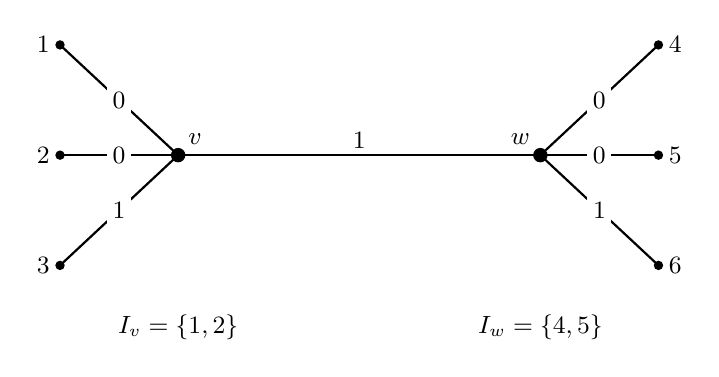
\begin{tikzpicture}[line cap=round,thick,every node/.style={font=\small},
 bit/.style={fill=white,inner sep=2pt}]
\coordinate (v) at (0,0);\coordinate (w) at (4.6,0);
\draw (v)--node[bit,above] {$1$}(w);
\foreach \name/\x/\y/\b in {1/-1.5/1.4/0,2/-1.5/0/0,3/-1.5/-1.4/1}{
 \draw (v)--node[bit] {$\b$}(\x,\y);
 \fill (\x,\y) circle(1.7pt);\node[left] at(\x,\y){$\name$};}
\foreach \name/\x/\y/\b in {4/6.1/1.4/0,5/6.1/0/0,6/6.1/-1.4/1}{
 \draw(w)--node[bit] {$\b$}(\x,\y);
 \fill(\x,\y)circle(1.7pt);\node[right]at(\x,\y){$\name$};}
\fill(v)circle(2.6pt);\fill(w)circle(2.6pt);
\node[above right]at(v){$v$};\node[above left]at(w){$w$};
\node[below]at(0,-1.9){$I_v=\{1,2\}$};
\node[below]at(4.6,-1.9){$I_w=\{4,5\}$};
\end{tikzpicture}

\caption{The net blocks for \eqref{cr:example}. Each leaf is an integral box; its edge label is the turn bit. The internal edge has bit one, so the two junctions stay separate. The direct leaves at the left junction fuse to $\{1,2\}$ and those at the right to $\{4,5\}$. Leaves $3,6$ are ordinary singleton blocks. These are label unions; no numerical zero test has been made.}\label{cr:net-figure}
\end{figure}

\subsection{An example and a zero wall}

Consider the explicit ordered expression
\begin{equation}\label{cr:example}
 C\bigl(R^{n_1}R^{n_2}h_3\,
                 \Turn(R^{n_4}R^{n_5}h_6)\bigr).
\end{equation}
It is in the original syntax since $R^{n_i}=\Turn h_i$. Put $a=n_1+n_2$ and $b=n_4+n_5$. Adjacent fusion gives
\[
                     C\bigl(R^a h_3\Turn(R^b h_6)\bigr).
\]
The partition is $\{1,2\},\{3\},\{4,5\},\{6\}$. The inner stack has type $HL=H$, its turn has type $L$, and the closing pair can be chosen $HA$. Thus the resulting formal expression is strict even on $a=0$ or $b=0$; the long-filling theorem applies only when its actual four weights are long.

On the wall $a=0$, removing the through identity is an additional evaluated move. The original rotations give
\begin{align*}
 C\bigl(h_3\Turn(R^b h_6)\bigr)
 &\simeq C\bigl(R^{n_3}\tau(R^b h_6)\bigr)\\
 &=C\bigl(R^{n_3}h_6R^b\bigr)
 \simeq C\bigl(R^{n_3+b}h_6\bigr).
\end{align*}
The surviving blocks have changed to $\{3,4,5\},\{6\}$, with $\{1,2\}$ deleted. The reversal $\tau(R^b h_6)=h_6R^b$ and final closed cyclic move are essential. This example explains why the zero-aware reduction needs a different finite partition statement.

\section{Zero pieces and the two-punctured cap sphere}\label{cr:zeros}

We now evaluate the weights. A zero integral box $R^0$ is the through identity, whereas
\[
                     h(0)=\Turn R^0
\]
is the cup-cap tangle. Interchanging them would give incorrect component counts. In a cylindrical product with at least two leaves, Lemma~\ref{cr:expose} puts a chosen zero ordinary leaf in the form $C(h(0)Q)$. Its two arcs are exactly the two caps of the other tangle, so
\begin{equation}\label{cr:zero-delete}
                         C(h(0)Q)\simeq D(Q).
\end{equation}
No isolated component is discarded in this isotopy.

\begin{lemma}[Cap splitting with its components]\label{cr:cap-split}
For arbitrary tangles $F,G$,
\begin{equation}\label{cr:cap-rules}
 D(\Turn F)\simeq C(\tau F),\qquad
 D(FG)\simeq D(F)\mathbin{\#}_{u_F,l_G}D(G).
\end{equation}
The subscripts specify the component containing the upper cap of $F$ and that containing the lower cap of $G$. The second equality is a componentwise connected sum exhibited by a sphere meeting the link in two points.
\end{lemma}
\begin{proof}
The first equality follows from \eqref{cr:two-closures}, retaining the actual half-turn. For the second, put the lower $F$ and upper $G$ in disjoint balls. Their interface consists of two short vertical arcs in an otherwise empty collar. Make the lower cap of $F$ and upper cap of $G$. A horizontal disk through the collar can be closed around the lower ball and its cap in the empty exterior. Its resulting sphere meets exactly the two interface arcs, once each, and no other component; see Figure~\ref{cr:closure-figure}.

Cut this sphere and cap its two punctures on each side by a trivial arc. The lower link is $D(F)$, with its new upper cap; the upper is $D(G)$, with its new lower cap. Rejoining those particular arcs recovers the original diagram. This proves the componentwise assertion as well as its reversibility. Internal closed components remain in their respective balls. A mark or ribbon is carried during the operation; nothing requires the upper and lower caps of a general tangle to lie on the same component.
\end{proof}

There are four elementary endings:
\begin{equation}\label{cr:endings}
\begin{array}{c|c}
\text{closure}&\text{actual link}\\\hline
C(R^s)&\text{the }(2,s)\text{ torus braid closure}\\
D(R^s)&\text{an unknot}\\
C(h(s))&D(R^s)\\
D(h(s))&C(R^s).
\end{array}
\end{equation}
For the last identity use $\tau R^s=R^s$. Every one-leaf expression reduces to one of these cases by shortening turn chains and resolving $\tau$ on that leaf. To see the second assertion, pull each successive braid crossing toward an end cap and remove the resulting curl. This is an unframed isotopy; a transported ribbon keeps the associated integer twists until the final framing correction. In particular $C(R^0)$ is the two-component unlink. A last zero box must be treated by \eqref{cr:endings} before applying any zero-deletion rule. There is no unspecified empty diagram at termination.

\subsection{The all-root algorithm}

Keep a closure flag $C$ or $D$ and the original attaching arcs with each pending factor. Give the one-box rule priority. A top turn changes $C(\Turn F)$ to $D(F)$; for $D(\Turn F)$ use \eqref{cr:cap-rules} and propagate $\tau$. A cap-closed product splits into its two children, both cap closed, with its specified connected-sum edge. A cylindrical product is normalized by Theorem~\ref{cr:ordered}. If the resulting strict factor has a zero net weight, expose that formal leaf by Lemma~\ref{cr:expose} and use \eqref{cr:zero-delete}; then continue. Apply the same rules separately in each pending factor. A definite traversal order makes every choice deterministic.

Every fusion or zero deletion decreases the number of live label blocks. Between such events, a top-turn reduction or cap splitting removes an operation vertex from the finite expression forest. Exposing one selected zero takes finitely many path steps and never copies a sibling. The normalization of a cylindrical product already terminates. These observations give termination by induction on the live-block count, with a finite amount of structural work between successive decreases. Each connected-sum edge is created by splitting one pending factor into two. Thus the recorded edges form a tree, and all subsequent moves take place in those factors with their attaching arcs retained.

At termination the strict factors have nonzero weights, the integral closures have their full integer exponents, and the cap closures in \eqref{cr:endings} are unknots. Deleting a zero block removes its live piece but records its original labels. Every other step either preserves a block or replaces disjoint blocks by their union. Surviving and deleted blocks therefore partition the original labels. This proves the topological part of Theorem~\ref{cr:arbitrary}.

\begin{proposition}[Finitely many evaluated templates]\label{cr:patterns}
For a fixed original expression, the all-root algorithm has only finitely many structural outputs. Each is fixed by
\begin{equation}\label{cr:pattern-data}
 \bigl(n_i\bmod2\bigr)_{i=1}^m,\qquad
 \bigl(\mathbf1_{W_B=0}\bigr)_{\varnothing\ne B\subseteq\{1,\ldots,m\}}.
\end{equation}
The ordered templates, their attaching components and their surviving/deleted blocks are constant on every realized pattern.
\end{proposition}
\begin{proof}
A rotation is determined by the parity of the moved sum. A deletion is determined by the vanishing of the current block weight. Rotations preserve crossing signs, fusion takes an ordinary sum and no step duplicates a label. Every integer quantity tested is therefore one of the subset sums in \eqref{cr:pattern-data}. With a fixed schedule, induction on the finite sequence of operations gives the assertion. There are at most $2^m2^{2^m-1}$ patterns, and unrealized patterns can be ignored. This crude bound is used only for finiteness.
\end{proof}

Tests for $s=1$ and $s=-1$ are not needed to choose these templates. They will be needed to decide which terminal elementary knots are trivial. Different additional zero relations can change the label partition, as the example in Section~\ref{cr:partition} shows.

\section{Components and the obstruction to two nontrivial factors}\label{cr:groups}

\subsection{What a one-component input implies}

The component bookkeeping is elementary and exact. At a product trace the joined strands, retain the pairing of the four remaining endpoints and record every new closed circle. At a turn permute the four endpoints. At closure add the cycles formed by its two closing arcs. An internal circle never rejoins a later endpoint.

For the connected-sum tree, if $c_v\ge1$ is the number of components of terminal factor $v$ and there are $r$ factors, Lemma~\ref{cr:cap-split} gives
\begin{equation}\label{cr:component-count}
               c(K)=\sum_v c_v-(r-1)
                    =1+\sum_v(c_v-1).
\end{equation}
It follows that a one-component input forces every terminal factor to be a knot. It also forbids an internal closed circle in a proper subtree of any terminal expression: that circle could never reconnect, while the four remaining endpoints eventually close to at least one further component. Thus the literal knot test required in Proposition~\ref{cr:import} is satisfied for each strict terminal factor.

Under its longness hypothesis, a strict terminal factor is a hyperbolic knot. A terminal elementary knot is either an unknot or a $(2,s)$ torus knot with odd $|s|\ge3$. The even braid closures, including $s=0$, are excluded by \eqref{cr:component-count}. We will use only these known kinds of factors; no primeness theorem for arbitrary short tangles is required.

\subsection{A meridian-centralizer calculation}

Write $X_K=S^3\setminus\operatorname{int}\nu K$ for a knot exterior, where $\nu K$ is a tubular neighborhood. A meridian $\mu$ has linking number one with the oriented knot and generates its infinite cyclic abelianization. Thus $\langle\mu\rangle\cong\mathbb Z$ injects into its group. Van Kampen on the meridional annulus of a connected sum gives
\begin{equation}\label{cr:amalgam}
 \pi_1(X_{K_1\#K_2})
       =\pi_1(X_{K_1})*_{\langle\mu\rangle}\pi_1(X_{K_2}).
\end{equation}
Transport the knot orientation through each attaching arc, so the meridians are identified consistently. If an inverse convention occurs, replacing that meridian by its inverse leaves the following centralizer argument unchanged.

We recall the group-theoretic fact used in \eqref{cr:amalgam}. Choose representatives of cosets of the common subgroup in each factor, including the identity. Moving subgroup elements across a syllable and collecting successive syllables from the same factor reduces a word to an alternating list of nonidentity coset representatives and a final subgroup element. The resulting lists define a group on which each factor acts by multiplication and reduction; the action obeys exactly the identifications of the common subgroup. In particular a nonempty reduced alternating list cannot represent the identity. This proves the injectivity of the factor maps and the usual reduced-word property of the amalgam. Iterating along the sum tree preserves each factor group. For $u,v$ in different factors, neither in $\langle\mu\rangle$, the word
\begin{equation}\label{cr:commutator}
                            uvu^{-1}v^{-1}
\end{equation}
is reduced and nontrivial.

\begin{lemma}[Commuting elements in the terminal groups]\label{cr:factors}
Every nontrivial terminal knot under the longness hypothesis has an element outside $\langle\mu\rangle$ commuting with its meridian.
\end{lemma}
\begin{proof}
For a hyperbolic factor, use its preferred longitude. The complete cusp is a quotient of a horoball by a rank-two translation lattice. In the faithful complete holonomy its peripheral group is $\mathbb Z^2$, so the longitude is not a power of the meridian and commutes with it.

For a $(2,s)$ torus knot, with odd $|s|\ge3$, the two solid tori on either side of the standard torus meet along the annulus left after removing the knot neighborhood. Its core winds twice around one solid-torus core and $s$ times around the other. Van Kampen gives
\begin{equation}\label{cr:torus-group}
                 G_s=\langle a,b\mid a^2=b^s\rangle,
                       \qquad z=a^2=b^s.
\end{equation}
The element $z$ commutes with both generators. Abelianization is infinite cyclic: with a generator $t$ one has $[a]=s t$, $[b]=2t$ and $[z]=2s t$. In particular $z$ is nontrivial, while a meridian has class $\pm t$.

The quotient by $\langle z\rangle$ is $C_2*C_{|s|}$, whose abelianization is cyclic of order $2|s|$. The image of a meridian generates that abelianization. A finite-order element of this free product is conjugate into one of its factors: a cyclically reduced word of length at least two has powers of strictly increasing reduced length. Its finite order would consequently divide $2$ or $|s|$, whereas the meridian's abelianization has order $2|s|$. The image of the meridian therefore has infinite order.

If $z=\mu^k$, abelianization forces $k=\pm2s\ne0$, contradicting that infinite order after quotienting by $z$. Thus the central element $z$ lies outside $\langle\mu\rangle$ and has the required property. This proof does not need a formula for the torus knot's preferred longitude.
\end{proof}

\begin{lemma}[Hyperbolic meridian centralizers]\label{cr:hyperbolic-centralizer}
In a complete finite-volume hyperbolic knot group the centralizer of a meridian is abelian and the center is trivial. Neither an unknot nor a nontrivial torus knot is a hyperbolic knot.
\end{lemma}
\begin{proof}
Faithful complete holonomy sends the meridian to a nontrivial parabolic. Conjugate it to $z\mapsto z+1$ on the Riemann sphere. A commuting M\"obius map fixes its unique fixed point $\infty$, so it is $z\mapsto az+b$. Commutation gives $a=1$. All such translations commute, proving the centralizer assertion.

If a nonidentity group element were central, the same calculation makes it a nontrivial translation. Commuting with it would then force the whole holonomy group to consist of translations. A discrete translation group has rank at most two. Its quotient of all of hyperbolic three-space has infinite volume: in the rank-two case an upper half-space fundamental region has a positive constant Euclidean horizontal area and volume proportional to $\int_0^\infty t^{-3}\,dt$; in lower rank the horizontal area is already infinite. This contradicts finite volume. The cyclic unknot group cannot be such a group either, since its meridian would generate a rank-one parabolic group. The nontrivial torus groups have the nonidentity center element from \eqref{cr:torus-group}, so they are excluded as well.
\end{proof}

\begin{proposition}[Selection of one strict factor]\label{cr:one-factor}
Under the longness hypothesis on all surviving strict factors, a hyperbolic input knot has exactly one strict terminal factor and all other terminal factors are unknots. It is ambient isotopic to that strict factor. Conversely this terminal configuration gives a hyperbolic input knot.
\end{proposition}
\begin{proof}
Every terminal factor is a knot by \eqref{cr:component-count}. If two are nontrivial, take their elements from Lemma~\ref{cr:factors}. Both commute with the common meridian in \eqref{cr:amalgam}, but their commutator is nontrivial by \eqref{cr:commutator}. This contradicts Lemma~\ref{cr:hyperbolic-centralizer}. There is at most one nontrivial factor.

If all factors are unknots, their iterated connected sum is an unknot. If the sole nontrivial factor is torus, the input is that torus knot. Both alternatives are excluded by the preceding lemma. The remaining possibility is exactly one long strict factor.

Connected sum with an exhibited unknot can be removed by straightening its summing arc across a spanning disk. One may take a spanning disk for the unknot closure and remove innermost intersections with the separating sphere; the remaining disk makes the arc in that ball boundary parallel. This is an ambient isotopy in the sum ball, and it preserves every other factor. Apply it successively along terminal edges of the sum tree. The input is thereby isotopic to the strict knot. Conversely that strict knot is hyperbolic by Proposition~\ref{cr:import}, and the same isotopies transport its metric to the input complement.
\end{proof}

\section{Uniform thresholds, invariant and volume}\label{cr:application}

For a fixed cylindrical product input, the symbolic normalization uses only the original parities. There are at most $2^m$ resulting ordered templates. For every strict one choose the crossing threshold \eqref{cr:crossing-threshold}, taking the maximum over its knot-producing parity choices if necessary. Define
\begin{equation}\label{cr:product-threshold}
 B(\mathcal E)=\max\bigl(\{2\}\cup
                \{B_\sigma:\sigma\text{ is a strict output}\}\bigr).
\end{equation}
If there is no strict output the maximum is simply $2$. For a knot with a strict output whose net weights exceed this number, Proposition~\ref{cr:import} supplies its complete hyperbolic metric and its invariant limit. The isotopies constructed above give the same conclusion for the input. This completes the second assertion of Theorem~\ref{cr:ordered}. If the input is already known to be hyperbolic, its elementary output is impossible by Lemma~\ref{cr:hyperbolic-centralizer}.

For either closure and the evaluated zero-aware reduction, Proposition~\ref{cr:patterns} gives a finite set $\mathcal S_E$ of possible strict terminal templates. Define
\begin{equation}\label{cr:all-threshold}
 B_E=\max\bigl(\{2\}\cup\{B_\sigma:\sigma\in\mathcal S_E\}\bigr).
\end{equation}
This threshold works simultaneously on every realized parity and subset-sum zero pattern of the fixed input. The construction is finite but does not provide a numerical value for the analytic thresholds in Proposition~\ref{cr:import}. There is no bound uniform over expressions with an increasing number of operations.

If the input has one component and its strict terminal weights exceed \eqref{cr:all-threshold}, Proposition~\ref{cr:one-factor} proves both directions of the hyperbolicity criterion in Theorem~\ref{cr:arbitrary}. For clarity, its terminal test is completely specified: $D(R^s)$ is always an unknot, and among knot closures $C(R^s)$ exactly $s=\pm1$ are unknots. Odd $|s|\ge3$ are the nontrivial torus factors in Lemma~\ref{cr:factors}. Even $s$ cannot occur for a one-component input. Thus the last classification step requires the two tests $s=\pm1$ in addition to the parity and zero tests which chose the templates.

\subsection{The same filled knot and its normalization}

Let the surviving strict knot be $K_*$. The reductions provide an orientation-preserving ambient isotopy of $S^3$ carrying the input knot to $K_*$. Carry a knot orientation, a marked point and a small tubular neighborhood along it. The resulting exterior homeomorphism sends a meridian to a meridian, since its disk still meets the core once, and sends the preferred longitude to the preferred longitude, since the primitive zero-linking condition is preserved. No extra meridional power is inserted into that longitude.

The reduced invariant of the same zero-framed knot is therefore exactly
\begin{equation}\label{cr:invariant}
                   K_N(K)=K_N(K_*),\qquad N\ge3.
\end{equation}
This uses the normalized knot invariant in Proposition~\ref{cr:import}, not an equality of two unnormalized colored sources. If intermediate ribbons are recorded, their transported framing can differ from the standard blackboard ribbon of the output by an integer. At complete color the twist is
\[
 \theta=q^{-d^2/2},\qquad q=e^{\pi\ii/N},\quad d=N-1,
                  \qquad |\theta|=1,
\]
by \cite[Theorem 10.1]{Finite}. Its integer power is removed by zero-framing and would in any case leave the exponential rate unchanged. The full one-cut modified convention, if chosen on both sides, retains its single factor $\ii^{N+3}/N$. Fusion does not create a modified dimension for each new twist region.

Pull back the strict knot's complete hyperbolic metric along the exterior homeomorphism. The resulting metric on the input complement has exactly the same volume. Equation~\eqref{cr:invariant} and Proposition~\ref{cr:import} prove \eqref{cr:volume-limit} for this original knot, completing Theorem~\ref{cr:arbitrary}. No connected-sum multiplicativity formula for the invariant, or additivity of its exponential rate, has been used.

The comparison is made after filling. Several filled boxes can fuse into a single box with a different auxiliary crossing circle. We have neither identified their unfilled augmented complements nor collapsed several independent quantum colors into one. The output strict presentation supplies its own actual primitive fillings; the already filled knots are the ones related by the constructed isotopy.

\subsection{Conditions directly on the original integers}

Theorem~\ref{cr:arbitrary} is strongest when the specified reduction is performed, because only its surviving strict weights are tested. There is also a convenient sufficient condition which does not require deciding which sums will survive.

\begin{corollary}[Separated nonzero subset sums]\label{cr:separated}
Fix $E$ and its closure. Suppose that for every nonempty original label set $B$,
\begin{equation}\label{cr:separated-formula}
                       W_B=0\quad\text{or}\quad|W_B|>B_E.
\end{equation}
Every hyperbolic knot given by that assignment satisfies \eqref{cr:volume-limit}. In particular, fix an integer vector $\mathbf a$ and put $\mathbf n=t\mathbf a$. For every fixed integer $t$ with $|t|>B_E$, each hyperbolic knot on this ray has the asserted limit.
\end{corollary}
\begin{proof}
Each surviving strict weight is a nonzero subset sum. Thus \eqref{cr:separated-formula} implies the exact longness condition of Theorem~\ref{cr:arbitrary}. On the ray, a nonzero sum is $t\sum_{i\in B}a_i$, whose magnitude is at least $|t|$. Zero entries and exact cancellations in $\mathbf a$ are allowed. The scale $t$ is fixed before $N$ tends to infinity.
\end{proof}

The corollary does not assert that every ray contains hyperbolic knots. The terminal criterion decides the alternative once the longness condition holds. A simpler sufficient case of \eqref{cr:separated-formula} is that all original nonzero counts have the same sign and magnitude greater than $B_E$.

If one writes the original counts as $n_i=\epsilon_i-2p_i$, a block has
\begin{equation}\label{cr:net-slope}
 W_B=\epsilon_B-2p_B,\qquad
 p_B=\sum_{i\in B}p_i+
             \frac{\epsilon_B-\sum_{i\in B}\epsilon_i}{2},
\end{equation}
where $\epsilon_B\in\{0,1\}$ has the parity of $W_B$. The correction is integral and fixed by the retained parity data. Independent longness of the original $p_i$ does not force longness of $p_B$ when signs cancel. The identity $R^a\simeq R^{a+2k}R^{-2k}$ is an actual example of this distinction, not a counterexample to a volume-conjecture equality.

\section{Finite reproduction and the limits of the reduction}\label{cr:reproduction}

The accompanying \texttt{check.py} uses only Python's standard library. From the repository root run
\[
 \texttt{python3 -I papers/conway-reductions/check.py}
\]
and optionally choose \texttt{--output /path/to/directory}.
The program removes an old summary before validation and records its input hashes. It checks the spatial rotation matrices and endpoint permutations, the compatibility of the closing reflection with a quarter-turn, and the arithmetic of the original label unions. It independently evaluates endpoint pairings and closed-component counts on finite expressions and compares the local sliding, closed-turn, cap-sum and zero-deletion identities. In these checks the closed components are retained; a control example shows that deleting a zero piece as a through identity changes the count. Further checks compare a parity-independent junction partition with a labelled symbolic reduction on bounded trees.

These are finite consistency tests of the conventions and bookkeeping. Endpoint pairings alone do not determine a tangle isotopy, and the checker makes no such inference. The actual isotopies are proved by the spatial collars, closing-sphere rotations and two-punctured cap spheres above. The tests do not prove the inherited analytic theorem or hyperbolic metric existence, nor do bounded trees prove termination for arbitrary size; the decreasing live-block argument does that.

The output is an exhibited reduction for one prescribed expression, not a prime decomposition or a classification of all presentations of the same knot. It can recognize more input expressions without enlarging the set of long strict knot types supplied by Proposition~\ref{cr:import}: each hyperbolic knot covered here is explicitly isotopic to one of those strict knots. Short surviving strict weights, growing expressions, pointed recurrence reconstruction and meridian or longitude asymptotics remain outside this paper.


\begin{thebibliography}{9}
\bibitem{Conway} J. H. Conway, \emph{An enumeration of knots and links, and some of their algebraic properties}, in Computational Problems in Abstract Algebra, Pergamon, 1970, 329--358. \href{https://doi.org/10.1016/B978-0-08-012975-4.50034-5}{doi:10.1016/B978-0-08-012975-4.50034-5}.
\bibitem{KL} L. H. Kauffman and S. Lambropoulou, \emph{On the classification of rational tangles}, Adv. Appl. Math. \textbf{33} (2004), 199--237. \href{https://doi.org/10.1016/j.aam.2003.06.002}{doi:10.1016/j.aam.2003.06.002}.
\bibitem{BS} F. Bonahon and L. C. Siebenmann, \emph{New Geometric Splittings of Classical Knots and the Classification and Symmetries of Arborescent Knots}, manuscript, version of January 26, 2016. \href{https://dornsife.usc.edu/francis-bonahon/wp-content/uploads/sites/205/2023/06/BonSieb-compressed.pdf}{Authors' edition}.
\bibitem{Volz} K. Reif Volz, \emph{Hyperbolicity of arborescent tangles and arborescent links}, Topology Appl. \textbf{156} (2009), 963--978. \href{https://doi.org/10.1016/j.topol.2008.11.014}{doi:10.1016/j.topol.2008.11.014}.
\bibitem{Profiles} \emph{Stationary profiles of strict Newton trees}. Companion paper, \href{https://sashakolpakov.github.io/murakamis_dream/papers/strict-newton-profiles.pdf}{repository edition}.
\bibitem{Asymptotics} \emph{Holomorphic source asymptotics and volume limits for strict Conway compositions}. Companion paper, \href{https://sashakolpakov.github.io/murakamis_dream/papers/conway-asymptotics.pdf}{repository edition}.
\bibitem{Finite} \emph{Finite spectral evaluation and uniform filling bounds}. Companion paper, \href{https://sashakolpakov.github.io/murakamis_dream/papers/filling-bounds.pdf}{repository edition}.
\end{thebibliography}
\end{document}
